%%%%%% Run at command line, run
%%%%%% xelatex grad-sample.tex 
%%%%%% for a few times to generate the output pdf file
\documentclass[12pt,oneside,openright,a4paper]{cpe-english-project}

\usepackage{polyglossia}
\setdefaultlanguage{english}
\setotherlanguage{thai}
\newfontfamily\thaifont[Script=Thai,Scale=1.23]{TH Sarabun New}
\defaultfontfeatures{Mapping=tex-text,Scale=1.0,LetterSpace=0.0}
\setmainfont[Scale=1.0,LetterSpace=0,WordSpace=1.0,FakeStretch=1.0]{Times New Roman}
\emergencystretch=10pt
%\XeTeXlinebreaklocale "th_TH"	
%\XeTeXlinebreakskip = 0pt plus 1pt
%\setmathfont(Digits)[Scale=1.0,LetterSpace=0,FakeStretch=1.0]{Times New Roman}


%%%%%%%%%%%%%%%%%%%%%%%%%%%%%%%%%%%%%%%%%%%%%%%%%%%%%%%%%%%%%%%%%%%
% Customize below to suit your needs 
% The ones that are optional can be left blank. 
%%%%%%%%%%%%%%%%%%%%%%%%%%%%%%%%%%%%%%%%%%%%%%%%%%%%%%%%%%%%%%%%%%%
% First line of title
\def\disstitleone{Project/Indep study title line 1}   
% Second line of title
\def\disstitletwo{Project/Indep title line 2 (optional)}   
% Your first name and lastname
\def\dissauthor{Mr./Ms. Firstname1 Lastname1}   % 1st member
%%% Put other group member names here ..
\def\dissauthortwo{Mr./Ms. Firstname2 Lastname2}   % 2nd member (optional)
\def\dissauthorthree{Mr./Ms. Firstname3 Lastname3}   % 3rd member (optional)


% The degree that you're persuing..
\def\dissdegree{Bachelor of Engineering} % Name of the degree
\def\dissdegreeabrev{B.Eng} % Abbreviation of the degree
\def\dissyear{202x}                   % Year of submission
\def\thaidissyear{256x}               % Year of submission (B.E.)

%%%%%%%%%%%%%%%%%%%%%%%%%%%%%%%%%%%%%%%%%%%%
% Your project and independent study committee..
%%%%%%%%%%%%%%%%%%%%%%%%%%%%%%%%%%%%%%%%%%%%
\def\dissadvisor{Assoc.Prof. My main advisor name , Ph.D.}  % Advisor
%%% Leave it empty if you have no Co-advisor
\def\disscoadvisor{Assoc.Prof. My Co-advisor name, Ph.D.}  % Co-advisor
%%% Leave it empty if you have no Co-advisor 2
\def\disscoadvisortwo{}  % Co-advisor 2 (if any)
\def\disscoadvisorthree{}  % Co-advisor 3 (You better be building space rocket or curing cancer at this point)
\def\disscommitteetwo{Asst.Prof. Committee2, Ph.D.}  % 3rd committee member (optional)
\def\disscommitteethree{Asst.Prof. Committee3, Ph.D.}   % 4th committee member (optional) 
\def\disscommitteefour{}    % 5th committee member (optional) 

\def\worktype{Project} %%  Project or Independent study
\def\disscredit{3}   %% 3 credits or 6 credits


\def\fieldofstudy{Computer Engineering} 
\def\department{Computer Engineering} 
\def\faculty{Engineering}

\def\thaifieldofstudy{วิศวกรรมคอมพิวเตอร์} 
\def\thaidepartment{วิศวกรรมคอมพิวเตอร์} 
\def\thaifaculty{วิศวกรรมศาสตร์}
 
\def\appendixnames{Appendix} %%% Appendices or Appendix

\def\thaiworktype{ปริญญานิพนธ์} %  Project or research project % 
\def\thaidisstitleone{หัวข้อปริญญานิพนธ์บรรทัดแรก}
\def\thaidisstitletwo{หัวข้อปริญญานิพนธ์บรรทัดสอง}
\def\thaidissauthor{นายสมศักดิ์ คอมพิวเตอร์}
\def\thaidissauthortwo{นางสาวสมศรี คอมพิวเตอร์2} %Optional
\def\thaidissauthorthree{นางสาวสมปอง คอมพิวเตอร์3} %Optional

\def\thaidissadvisor{รศ.ดร.ที่ปรึกษา วิทยานิพนธ์}
%% Leave this empty if you have no co-advisor
\def\thaidisscoadvisor{รศ.ดร.ที่ปรึกษา วิทยานิพนธ์ร่วม} %Optional
\def\thaidisscoadvisortwo{}  % Co-advisor 2 (if any)
\def\thaidisscoadvisorthree{} % Co-advisor 3 (You better be building space rocket or curing cancer at this point)
\def\thaidissdegree{วิศวกรรมศาสตรบัณฑิต}

% Change the line spacing here...
\linespread{1.15}

%%%%%%%%%%%%%%%%%%%%%%%%%%%%%%%%%%%%%%%%%%%%%%%%%%%%%%%%%%%%%%%%
% End of personal customization.  Do not modify from this part 
% to \begin{document} unless you know what you are doing...
%%%%%%%%%%%%%%%%%%%%%%%%%%%%%%%%%%%%%%%%%%%%%%%%%%%%%%%%%%%%%%%%


%%%%%%%%%%%% Dissertation style %%%%%%%%%%%
%\linespread{1.6} % Double-spaced  
%%\oddsidemargin    0.5in
%%\evensidemargin   0.5in
%%%%%%%%%%%%%%%%%%%%%%%%%%%%%%%%%%%%%%%%%%%
%\renewcommand{\subfigtopskip}{10pt}
%\renewcommand{\subfigbottomskip}{-5pt} 
%\renewcommand{\subfigcapskip}{-6pt} %vertical space between caption
%                                    %and figure.
%\renewcommand{\subfigcapmargin}{0pt}

\renewcommand{\topfraction}{0.85}
\renewcommand{\textfraction}{0.1}

\newtheorem{theorem}{Theorem}
\newtheorem{lemma}{Lemma}
\newtheorem{corollary}{Corollary}

\def\QED{\mbox{\rule[0pt]{1.5ex}{1.5ex}}}
\def\proof{\noindent\hspace{2em}{\itshape Proof: }}
\def\endproof{\hspace*{\fill}~\QED\par\endtrivlist\unskip}
%\newenvironment{proof}{{\sc Proof:}}{~\hfill \blacksquare}
%% The hyperref package redefines the \appendix. This one 
%% is from the dissertation.cls
%\def\appendix#1{\iffirstappendix \appendixcover \firstappendixfalse \fi \chapter{#1}}
%\renewcommand{\arraystretch}{0.8}
%%%%%%%%%%%%%%%%%%%%%%%%%%%%%%%%%%%%%%%%%%%%%%%%%%%%%%%%%%%%%%%%
%%%%%%%%%%%%%%%%%%%%%%%%%%%%%%%%%%%%%%%%%%%%%%%%%%%%%%%%%%%%%%%%


\begin{document}
\pdfstringdefDisableCommands{%
\let\MakeUppercase\relax
}
\begin{center}
  
\includegraphics[width=2.8cm]{logo02.jpg}
\end{center}
\vspace*{-1cm}

\maketitlepage
\makesignaturepage 

%%%%%%%%%%%%%%%%%%%%%%%%%%%%%%%%%%%%%%%%%%%%%%%%%%%%%%%%%%%%%%
%%%%%%%%%%%%%%%%%%%%%% English abstract %%%%%%%%%%%%%%%%%%%%%%%
%%%%%%%%%%%%%%%%%%%%%%%%%%%%%%%%%%%%%%%%%%%%%%%%%%%%%%%%%%%%%%
\abstract

In a multihop ad hoc network, the interference among nodes is
  reduced to maximize the throughput by using a smallest transmission
  range that still preserve the network connectivity. However, most
  existing works on transmission range control focus on the
  connectivity but lack of results on the throughput performance. This
  paper analyzes the per-node saturated throughput of an IEEE 802.11b
  multihop ad hoc network with a uniform transmission range. Compared
  to simulation, our model can accurately predict the per-node
  throughput.  The results show that the maximum achievable per-node
  throughput can be as low as 11\% of the channel capacity in a normal
  set of $\alpha$ operating parameters independent of node density. However, if
  the network connectivity is considered, the obtainable throughput
  will reduce by as many as 43\% of the maximum throughput. 

\begin{flushleft}
\begin{tabular*}{\textwidth}{@{}lp{0.8\textwidth}}
\textbf{Keywords}: & Multihop ad hoc networks / Topology control / Single-Hop Throughput
\end{tabular*}
\end{flushleft}
\endabstract

%%%%%%%%%%%%%%%%%%%%%%%%%%%%%%%%%%%%%%%%%%%%%%%%%%%%%%%%%%%%%%
%%%%%%%%%% Thai abstract here %%%%%%%%%%%%%%%%%%%%%%%%%%%%%%%%%
%%%%%%%%%%%%%%%%%%%%%%%%%%%%%%%%%%%%%%%%%%%%%%%%%%%%%%%%%%%%%%
{
%\begin{thai}
\XeTeXlinebreaklocale "th_TH"	
\XeTeXlinebreakskip = 0pt plus 1pt
\thaifont
\thaiabstract

การวิจัยครั้งนี้มีวัตถุประสงค์  เพื่อศึกษาความพึงพอใจในการให้บริการงานทั่วไปของสานักวิชา พื้นฐานและภาษา เพื่อเปรียบเทียบระดับความพึงพอใจต่อการให้บริการงาน ทั่วไปของสานักวิชาพื้นฐานและภาษา ของนักศึกษาที่มาใช้บริการสานักวิชาพื้นฐานและภาษา สถาบัน เทคโนโลยีไทย-ญี่ปุ่น จาแนกตามเพศ คณะ และชั้นปีที่ศึกษา เพื่อศึกษาปัญหาและข้อเสนอแนะของ นักศึกษามาเป็นแนวทางในการพัฒนาและปรับปรุงการให้บริการของสานักวิชาพื้นฐานและภาษา
เนื่องจากในยุคสมัยนี้โลกเราได้เข้าสู่ยุคของข้อมูลมหัต (Big data) ซึ่งบริษัทต่าง ๆก็เริ่มขับเคลื่อนธุรกิจด้วยข้อมูลแล้ว  โดยธุรกิจที่มีข้อมูลขนาดใหญ่อย่างที่เห็นง่ายๆเลยก็จะเป็น เว็บไซต์ที่เปิดบริการให้ขายของออนไลน์ ซึ่งในเว็บไซต์นั้นก็จะมีข้อมูลสินค้ามากมายและ สิ่งที่เราได้พบคือรายละเอียดสินค้าหลายๆอย่างไม่มีความสอดคล้องกับรูปภาพสินค้าหรือไม่ชัดเจนพอและ เนื่องด้วยข้อมูลที่มีขนาดใหญ่เกินกว่าที่จะจัดการด้วยแรงงานคนได้และ ยังไม่มีเครื่องมือใด ๆ ในการตรวจจับคำผิดเหล่านี้ได้ เราจึงทำโครงงานนี้ขึ้นมาเพื่อที่จะแก้ไขปัญหาเหล่านี้\par
ทางเราจึงคิดที่จะทำระบบปัญญาประดิษฐ์หรือ AI มาแก้ไขปัญหาในส่วนนี้ โดยทำ Image captioning ที่ใช้ Convolutional neural network และ Long short-term memory ซึ่งทางคณะผู้จัดทำก็จะมีการเปรียบเทียบกับสถาปัตยกรรมของโมเดลอื่น ๆ เพื่อสร้างโมเดลที่มีประสิทธิภาพมากที่สุด ซึ่งถ้าโครงงานนี้ประสบความสำเร็จจะสามารถตรวจสอบคุณภาพของคำอธิบายสินค้าในเว็บไซต์ขายสินค้าออนไลน์ ทำให้คุณภาพและภาพลักษณ์ต่อสังคมของเว็บไซต์นั้นดูดีขึ้นได้ และนอกจากนี้โครงงานนี้ยังสามารถเป็นพื้นฐานให้แก่ผู้ที่สนใจในการทำ image captioning ที่เป็นภาษาไทยและนำไปประยุกต์ใช้กับงานของตนได้อีกด้วย 

\begin{flushleft}
\begin{tabular*}{\textwidth}{@{}lp{0.8\textwidth}}
 & \\

\textbf{คำสำคัญ}: & การชุบเคลือบด้วยไฟฟ้า / การชุบเคลือบผิวเหล็ก /  เคลือบผิวรังสี
\end{tabular*}
\end{flushleft}
\endabstract
%\end{thai}
}

%%%%%%%%%%%%%%%%%%%%%%%%%%%%%%%%%%%%%%%%%%%%%%%%%%%%%%%%%%%%
%%%%%%%%%%%%%%%%%%%%%%% Acknowledgments %%%%%%%%%%%%%%%%%%%%
%%%%%%%%%%%%%%%%%%%%%%%%%%%%%%%%%%%%%%%%%%%%%%%%%%%%%%%%%%%%
\preface
Acknowledge your advisors and thanks your friends here..

%%%%%%%%%%%%%%%%%%%%%%%%%%%%%%%%%%%%%%%%%%%%%%%%%%%%%%%%%%%%%
%%%%%%%%%%%%%%%% ToC, List of figures/tables %%%%%%%%%%%%%%%%
%%%%%%%%%%%%%%%%%%%%%%%%%%%%%%%%%%%%%%%%%%%%%%%%%%%%%%%%%%%%%
% The three commands below automatically generate the table 
% of content, list of tables and list of figures
\tableofcontents                    
\listoftables
\listoffigures                      

%%%%%%%%%%%%%%%%%%%%%%%%%%%%%%%%%%%%%%%%%%%%%%%%%%%%%%%%%%%%%%
%%%%%%%%%%%%%%%%%%%%% List of symbols page %%%%%%%%%%%%%%%%%%%
%%%%%%%%%%%%%%%%%%%%%%%%%%%%%%%%%%%%%%%%%%%%%%%%%%%%%%%%%%%%%%
% You have to add this manually..
\listofsymbols
\begin{flushleft}
\begin{tabular}{@{}p{0.07\textwidth}p{0.7\textwidth}p{0.1\textwidth}}
\textbf{SYMBOL}  & & \textbf{UNIT} \\[0.2cm]
$\alpha$ & Test variable\hfill & m$^2$ \\
$\lambda$ & Interarival rate\hfill &  jobs/second\\
$\mu$ & Service rate\hfill & jobs/second\\
\end{tabular}
\end{flushleft}
%%%%%%%%%%%%%%%%%%%%%%%%%%%%%%%%%%%%%%%%%%%%%%%%%%%%%%%%%%%%%%
%%%%%%%%%%%%%%%%%%%%% List of vocabs & terms %%%%%%%%%%%%%%%%%
%%%%%%%%%%%%%%%%%%%%%%%%%%%%%%%%%%%%%%%%%%%%%%%%%%%%%%%%%%%%%%
% You also have to add this manually..
\listofvocab
\begin{flushleft}
\begin{tabular}{@{}p{1in}@{=\extracolsep{0.5in}}p{0.73\textwidth}}
ABC & Adaptive Bandwidth Control \\
MANET & Mobile Ad Hoc Network  \\
Test & Lorem ipsum dolor sit amet, consectetur adipiscing elit. Nullam non condimentum purus. Pellentesque sed augue sapien. In volutpat quis diam laoreet suscipit. Curabitur fringilla sem nisi, at condimentum lectus consequat vitae.
\end{tabular}
\end{flushleft}

%\setlength{\parskip}{1.2mm}

%%%%%%%%%%%%%%%%%%%%%%%%%%%%%%%%%%%%%%%%%%%%%%%%%%%%%%%%%%%%%%%
%%%%%%%%%%%%%%%%%%%%%%%% Main body %%%%%%%%%%%%%%%%%%%%%%%%%%%%
%%%%%%%%%%%%%%%%%%%%%%%%%%%%%%%%%%%%%%%%%%%%%%%%%%%%%%%%%%%%%%%


\chapter{Introduction}

THIS IS AN EXAMPLE. ALL SECTIONS BELOW ARE OPTIONAL. PLEASE CONSULT YOU ADVISOR AND DESIGN YOUR OWN SECTION

\emph{\textthai{หัวข้อต่าง ๆ ในแต่ละบทเป็นเพียงตัวอย่างเท่านั้น หัวข้อที่จะใส่ในแต่ละบทขึ้นอยู่กับโปรเจคของนักศึกษาและอาจารย์ที่ปรึกษา}}


\section{Background} 

Lorem ipsum dolor sit amet, consectetur adipiscing elit. Sed maximus sem id nisi imperdiet commodo. Vestibulum ante ipsum primis in faucibus orci luctus et ultrices posuere cubilia curae; Morbi sed dignissim nunc. Sed gravida semper porta. Maecenas scelerisque ex viverra ipsum condimentum pulvinar. Quisque auctor est nec venenatis accumsan. Phasellus finibus tincidunt blandit. Donec ac ante lectus. Mauris facilisis aliquet lorem quis imperdiet. Aenean pretium enim et placerat ultrices. Suspendisse tempor elit et imperdiet mattis. Vivamus quis lacus congue, efficitur augue vel, consequat eros. Aenean consequat risus ut consectetur convallis. Suspendisse convallis, ligula id pretium efficitur, tellus nunc commodo neque, et scelerisque lacus arcu quis orci. Donec tempor massa leo, ac sodales magna molestie ut. Quisque id interdum ante.

Explain the background of your works for readers. You can refer to figure by like this.. Figure~\ref{fig:x1}.
Get ready, skanks! It's time for the truth train! Fame was like a drug. But what was even more like a drug were the drugs. Attempted murder? Now honestly, what is that? Do they give a Nobel Prize for attempted chemistry?

\textthai{ทดสอบ}

\begin{figure}[!h]
\centering
\fbox{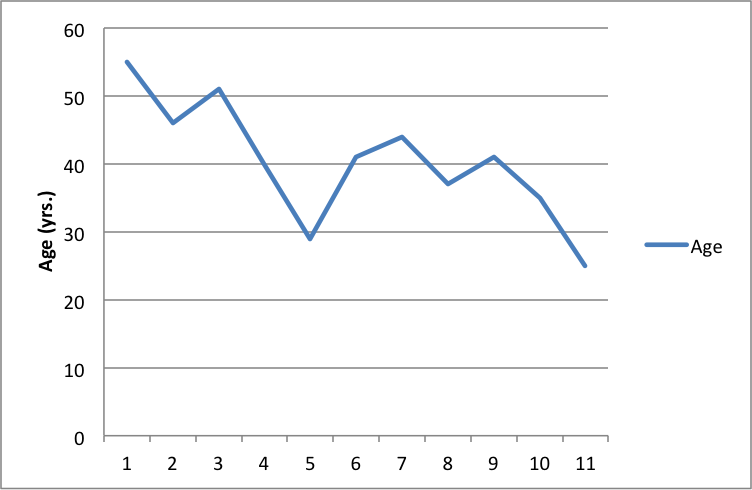
\includegraphics[width=10cm]{./chart-figure-5.png}}
\caption{This is the figure x1}\label{fig:chart-figure-5}
\end{figure}

Get ready, skanks! It's time for the truth train! Fame was like a drug. But what was even more like a drug were the drugs. Attempted murder? Now honestly, what is that? Do they give a Nobel Prize for attempted chemistry?

"Thank the Lord"? That sounded like a prayer. A prayer in a public school. God has no place within these walls, just like facts don't have a place within an organized religion. Thank you, steal again. I hope this has taught you kids a lesson: kids never learn.

…And the fluffy kitten played with that ball of string all through the night. On a lighter note, a Kwik-E-Mart clerk was brutally murdered last night. Oh, so they have Internet on computers now!

You don't like your job, you don't strike. You go in every day and do it really half-assed. That's the American way. Lisa, vampires are make-believe, like elves, gremlins, and Eskimos. Jesus must be spinning in his grave!

I prefer a vehicle that doesn't hurt Mother Earth. It's a go-cart, powered by my own sense of self-satisfaction. Marge, it takes two to lie. One to lie and one to listen. Attempted murder? Now honestly, what is that? Do they give a Nobel Prize for attempted chemistry?

I was saying "Boo-urns." Bart, with \$10,000 we'd be millionaires! We could buy all kinds of useful things like…love! I'll keep it short and sweet — Family. Religion. Friendship. These are the three demons you must slay if you wish to succeed in business.

How could you?! Haven't you learned anything from that guy who gives those sermons at church? Captain Whatshisname? We live in a society of laws! Why do you think I took you to all those Police Academy movies? For fun? Well, I didn't hear anybody laughing, did you? Except at that guy who made sound effects. Makes sound effects and laughs. Where was I? Oh yeah! Stay out of my booze. I can't go to juvie. They use guys like me as currency.

Oh, loneliness and cheeseburgers are a dangerous mix. "Thank the Lord"? That sounded like a prayer. A prayer in a public school. God has no place within these walls, just like facts don't have a place within an organized religion.


\section{Motivations}
Explain the motivations of your works.  
\begin{itemize}
\item   What are the problems you are addressing? 
\item  Why they are important?
\item  What are the limitations of existing approaches? 
\end{itemize}
You may combine this section with the background section.


\section{Problem Statements}

\section{Objectives}

\section{Scope of Work}

Explain the scope of your works. 
\begin{itemize}
\item   What are the problems you are addressing? 
\item  Why they are important?
\item  What are the limitations of existing approaches? 
\end{itemize}

\section{Project Schedule}

%%%%%%%%%%%%%%%%%%%%%%%%%%%%%%%%%%%%%%%%%%%%%%%%%%%%%%%%%%%%
%%%%%%%%%%%%%%  Literature Review %%%%%%%%%%%%%%%%%%%%%%%%%%
%%%%%%%%%%%%%%%%%%%%%%%%%%%%%%%%%%%%%%%%%%%%%%%%%%%%%%%%%%%%
\chapter{Background Theory and Related Work}

THIS IS AN EXAMPLE. ALL SECTIONS BELOW ARE OPTIONAL. PLEASE CONSULT YOU ADVISOR AND DESIGN YOUR OWN SECTION

\emph{\textthai{หัวข้อต่าง ๆ ในแต่ละบทเป็นเพียงตัวอย่างเท่านั้น หัวข้อที่จะใส่ในแต่ละบทขึ้นอยู่กับโปรเจคของนักศึกษาและอาจารย์ที่ปรึกษา}}

This is how you add website url. -> \url{http://www.cpe.kmutt.ac.th}

Explain theory, algorithms, protocols, or existing research works and tools related to your work.

You can cite your references like this -> \cite{santi05b}  or multiplie cite like this -> \cite{bworld,hypersense}

\section{Recommender Systems}

\begin{table}[!h]
\caption{test table method1}\label{tbl:method1}
\begin{tabular}{c|c|l|rr} \hline\hline
Center & Center & left aligned & Right & Right aligned \\ \hline\hline
Center & Center & left aligned & Right & Right aligned \\ \hline
Center & Center & left aligned & Right & Right aligned \\ 
Center & Center & left aligned & Right & Right aligned \\ \hline
Center & Center & left aligned & Right & Right aligned \\ \hline\hline
\end{tabular}
\end{table}

Tables should always on the left.
\section{Text Processing Algorithms}
\subsection{Algorithm I}
\subsubsection{test}

% Can define this in the preamble..
You can place the figure and refer to it as Figure~\ref{fig:model2}.
The figure and table numbering will be run and updated automatically when you add/remove tables/figures from the document.

\begin{figure}[!h]\centering
\setlength{\fboxrule}{0.2mm} % can define this in the preamble
\setlength{\fboxsep}{1cm}
\fbox{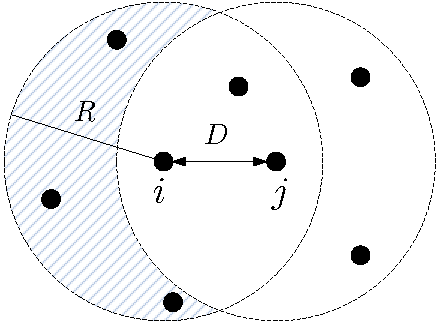
\includegraphics[width=5cm]{./model2.pdf}}
\caption{The network model}\label{fig:model2}
\end{figure}

 
\subsection{Algorithm II}
Add more subsections as you want.
\subsubsection{Step I}
\subsubsection{Step II}
This is the farthest level of subsection we permitted. (We support only 4th level)

\section{Development Tools}

%%%%%%%%%%%%%%%%%%%%%%%%%%%%%%%%%%%%%%%%%%%%%%%%%%%%%55
%%%%%%%%%%%%%%%%%%%%%%%%%%%%%%%%%%%%%%%%%%%%%%%%%%%%%
%%%%%%%%%%%%%%%%%%%%%%%%%%%%%%%%%%%%%%%%%%%%%%%%%%%%%
\chapter{Proposed Work}


THIS IS AN EXAMPLE. ALL SECTIONS BELOW ARE OPTIONAL. PLEASE CONSULT YOU ADVISOR AND DESIGN YOUR OWN SECTION

\emph{\textthai{หัวข้อต่าง ๆ ในแต่ละบทเป็นเพียงตัวอย่างเท่านั้น หัวข้อที่จะใส่ในแต่ละบทขึ้นอยู่กับโปรเจคของนักศึกษาและอาจารย์ที่ปรึกษา}}


Explain the design (how you plan to implement your work) of your project. Adjust the section titles below to suit the types of your work. Detailed physical design like circuits and source codes should be placed in the appendix.

\section{System Architecture}

\begin{table}[!h]
\centering
\caption{test table x1}\label{tbl:symbols}
\begin{tabular}{@{}p{0.07\textwidth}|p{0.7\textwidth}p{0.1\textwidth}}\hline
\multicolumn{2}{l}{\textbf{SYMBOL}}  & \textbf{UNIT} \\ \hline 
$\alpha$ & Test variable\hfill & m$^2$ \\
$\lambda$ & Interarrival rate\hfill &  jobs/second\\
$\mu$ & Service rate\hfill & jobs/second \\ \hline
\end{tabular}
%\begin{tabular}{c|c} \hline
% $\alpha$ & $\beta$ \\ \hline
% $\delta$ & $\mu$ \\ \hline
%\end{tabular}
\end{table}

\section{System Specifications and Requirements}

\section{Hardware Module 1}
\subsection{Component 1}
\subsection{Logical Circuit Diagram}

\section{Hardware Module 2}
\subsection{Component 1}
\subsection{Component 2}

\section{Path Finding Algorithm}

\section{Database Design}

\section{GUI Design}



%%%%%%%%%%%%%%%%%%%%%%%%%%%%%%%%%%%%%%%%%%%%%%%%%%%%%%%%%%%%%%
%%%%%%%%%%%%%%%%%%%% Experiments %%%%%%%%%%%%%%%%%%%%%%%%%%%%%
%%%%%%%%%%%%%%%%%%%%%%%%%%%%%%%%%%%%%%%%%%%%%%%%%%%%%%%%%%%%%%%
\chapter{Implementation Results}

You can title this chapter as \textbf{Preliminary Results} or \textbf{Work Progress} for the progress reports. Present implementation or experimental results here and discuss them.


ALL SECTIONS IN THIS CHAPTER ARE OPTIONAL. PLEASE CONSULT YOU ADVISOR AND DESIGN YOUR OWN SECTION

\emph{\textthai{หัวข้อต่าง ๆ ในแต่ละบทเป็นเพียงตัวอย่างเท่านั้น หัวข้อที่จะใส่ในแต่ละบทขึ้นอยู่กับโปรเจคของนักศึกษาและอาจารย์ที่ปรึกษา}}

%%%%%%%%%%%%%%%%%%%%%%%%%%%%%%%%%%%%%%%%%%%%%%%%%%%%%%%%%%%%%%%
%%%%%%%%%%%%%%%%%%%% Conclusions %%%%%%%%%%%%%%%%%%%%%%%%%%%%%
%%%%%%%%%%%%%%%%%%%%%%%%%%%%%%%%%%%%%%%%%%%%%%%%%%%%%%%%%%%%%%%
\chapter{Conclusions}

 \begin{figure}[!h]
\caption{This is how you mention when figure come from internet  \href{https://www.google.com} {https://www.google.com}}\label{fig:x1}
\end{figure}

This chapter is optional for proposal and progress reports but 
is required for the final report.

THIS IS AN EXAMPLE. ALL SECTIONS BELOW ARE OPTIONAL. PLEASE CONSULT YOU ADVISOR AND DESIGN YOUR OWN SECTION

\emph{\textthai{หัวข้อต่าง ๆ ในแต่ละบทเป็นเพียงตัวอย่างเท่านั้น หัวข้อที่จะใส่ในแต่ละบทขึ้นอยู่กับโปรเจคของนักศึกษาและอาจารย์ที่ปรึกษา}}

\section{Problems and Solutions}
State your problems and how you fixed them.

\section{Future Works}
What could be done in the future to make your projects better.

%%%%%%%%%%%%%%%%%%%%%%%%%%%%%%%%%%%%%%%%%%%%%%%%%%%%%%%%%%%%%%%
%%%%%%%%%%%%%%%%%%%% Bibliography %%%%%%%%%%%%%%%%%%%%%%%%%%%%%
%%%%%%%%%%%%%%%%%%%%%%%%%%%%%%%%%%%%%%%%%%%%%%%%%%%%%%%%%%%%%%%

%%%% Comment this in your report to show only references you have
%%%% cited. Otherwise, all the references below will be shown.
%\nocite{*}
%% Use the kmutt.bst for bibtex bibliography style 
%% You must have cpe.bib and string.bib in your current directory.
%% You may go to file .bbl to manually edit the bib items.

% Sept, 2021 by Thanin
% improve url breaks to prevent unnecessary big white spaces in some cases
\makeatletter
\g@addto@macro{\UrlBreaks}{\UrlOrds}
\makeatother
% 

\bibliographystyle{kmutt}
\bibliography{string,cpe}

%%%%%%%%%%%%%%%%%%%%%%%%%%%%%%%%%%%%%%%%%%%%%%%%%%%%%%%%%%%%%%%
%%%%%%%%%%%%%%%%%%%%%%%% Appendix %%%%%%%%%%%%%%%%%%%%%%%%%%%%%
%%%%%%%%%%%%%%%%%%%%%%%%%%%%%%%%%%%%%%%%%%%%%%%%%%%%%%%%%%%%%%%
\appendix{First appendix title}
\noindent{\large\bf Put appropriate topic here} \\

This is where you put hardware circuit diagrams, detailed experimental data in tables or source codes, etc.. \\ \bigskip

 \begin{figure}[!h]
\caption{This is the figure x11 \href{https://www.google.com} {https://www.google.com}}\label{fig:x1}
\end{figure}

This appendix describes two static allocation methods for fGn (or fBm)
traffic. Here, $\lambda$ and $C$ are respectively the traffic arrival
rate and the service rate per dimensionless time step. Their unit are
converted to a physical time unit by multiplying the step size
$\Delta$. For a fBm self-similar traffic source,
Norros~\cite{norros95} provides its EB as
\begin{equation}\label{eq:norros}
  C = \lambda + (\kappa(H)\sqrt{-2\ln\epsilon})^{1/H}a^{1/(2H)}x^{-(1-H)/H}\lambda^{1/(2H)}
\end{equation}
where $\kappa(H) = H^H(1-H)^{(1-H)}$. Simplicity in the calculation is
the attractive feature of (\ref{eq:norros}).

The MVA technique developed in~\cite{kim01} so far provides the most
accurate estimation of the loss probability compared to previous
bandwidth allocation techniques according to simulation results.
Consider a discrete-time queueing system with constant service rate
$C$ and input process $\lambda_n$ with $\mathbb{E}\{\lambda_n\} =
\lambda$ and $\mathrm{Var}\{\lambda_n\} = \sigma^2$.  Define $X_n \equiv
\sum_{k=1}^n \lambda_k - Cn$.  The loss probability due to the MVA
approach is given by
\begin{equation}\label{eq:loss_mva}
  \varepsilon \approx \alpha e^{-m_x/2}
\end{equation}
where
\begin{equation}\label{eq:mx}
m_x = \min_{n \geq 0} \frac{((C-\lambda)n + B)^2}{\mathrm{Var}\{X_n\}} =
\frac{((C-\lambda)n^\ast + B)^2}{\mathrm{Var}\{X_{n^{\ast}}\}}
\end{equation} 
and 
\begin{equation}\label{eq:alpha}
  \alpha =
  \frac{1}{\lambda\sqrt{2\pi\sigma^2}}\exp\left(\frac{(C-\lambda)^2}{2\sigma^2}\right)
  \int_C^\infty (r-C)\exp\left(\frac{(r-\lambda)^2}{2\sigma^2}\right)\, dr
\end{equation}
For a given $\varepsilon$, we numerically solve for $C$ that satisfies
(\ref{eq:loss_mva}). Any search algorithm can be used to do the task.
Here, the bisection method is used.  

Next, we show how $\mathrm{Var}\{X_n\}$ can be determined.  Let
$C_{\lambda}(l)$ be the autocovariance function of $\lambda_n$.  The
MVA technique basically approximates the input process $\lambda_n$
with a Gaussian process, which allows $\mathrm{Var}\{X_n\}$ to be
represented by the autocovariance function.  In particular, the
variance of $X_n$ can be expressed in terms of $C_{\lambda}(l)$ as
\begin{equation}
  \mathrm{Var}\{X_n\} = nC_{\lambda}(0) + 2\sum_{l=1}^{n-1} (n-l)C_{\lambda}(l)
\end{equation} 
Therefore, $C_{\lambda}(l)$ must be known in the MVA technique, either
by assuming specific traffic models or by off-line analysis in case of
traces.  In most practical situations, $C_{\lambda}(l)$ will not be
known in advance, and an on-line measurement algorithm developed
in~\cite{eun01} is required to jointly determine both $n^\ast$ and
$m_x$. For fGn traffic, $\mathrm{Var}\{X_n\}$ is equal to $\sigma^2
n^{2H}$, where $\sigma^2 = \mathrm{Var}\{\lambda_n\}$, and we can find
the $n^\ast$ that minimizes (\ref{eq:mx}) directly. Although $\lambda$
can be easily measured, it is not the case for $\sigma^2$ and $H$.
Consequently, the MVA technique suffers from the need of prior
knowledge traffic parameters.


%%%%%%%%%%%%%%%%%%%%%%%%%%%%%%%%%%%%%%%%%%%%%%%%%%%%%%%%%%
%%%%%%%%%%%%%%% The 2nd appendix %%%%%%%%%%%%%%%%%%%%%%%%%%
%%%%%%%%%%%%%%%%%%%%%%%%%%%%%%%%%%%%%%%%%%%%%%%%%%%%%%%%%%
\appendix{Second appendix title}
\noindent{\large\bf Put appropriate topic here} \\


 \begin{figure}[!h]
\caption{This is the figure x11 \href{https://www.google.com} {https://www.google.com}}\label{fig:x1}
\end{figure}

Next, we show how $\mathrm{Var}\{X_n\}$ can be determined.  Let
$C_{\lambda}(l)$ be the autocovariance function of $\lambda_n$.  The
MVA technique basically approximates the input process $\lambda_n$
with a Gaussian process, which allows $\mathrm{Var}\{X_n\}$ to be
represented by the autocovariance function.  In particular, the
variance of $X_n$ can be expressed in terms of $C_{\lambda}(l)$ as
\begin{equation}
  \mathrm{Var}\{X_n\} = nC_{\lambda}(0) + 2\sum_{l=1}^{n-1} (n-l)C_{\lambda}(l)
\end{equation} 

\noindent{\large\bf Add more topic as you need} \\

Therefore, $C_{\lambda}(l)$ must be known in the MVA technique, either
by assuming specific traffic models or by off-line analysis in case of
traces.  In most practical situations, $C_{\lambda}(l)$ will not be
known in advance, and an on-line measurement algorithm developed
in~\cite{eun01} is required to jointly determine both $n^\ast$ and
$m_x$. For fGn traffic, $\mathrm{Var}\{X_n\}$ is equal to $\sigma^2
n^{2H}$, where $\sigma^2 = \mathrm{Var}\{\lambda_n\}$, and we can find
the $n^\ast$ that minimizes (\ref{eq:mx}) directly. Although $\lambda$
can be easily measured, it is not the case for $\sigma^2$ and $H$.
Consequently, the MVA technique suffers from the need of prior
knowledge traffic parameters. 





\end{document}
